\section{Methods}
\subsection{Data Collection}
multiple runs, average of every node
\subsection{Metrics}
For each graph, the x axis signifies number of epochs of training, and the y axis signifies accuracy. Accuracy is calculated after the synchronisation step, by checking the number of correct predictions on an unseen test set.
\subsection{Node Counts}
All experiment use 10 nodes unless otherwise stated. All experiments show the average accuracy of each 10 nodes x 5 experiments = 50 nodes

\section{Experiments}
\subsection{Combination Methods: Averaging vs Averaging with Synchronisation Rate}
The purpose of this experiment was to compare the effectiveness of \emph{averaging} (\emph{AVG}) to \emph{averaging with synchronisation rate} (\emph{ASR}). Below are some details of the experiment:

\begin{itemize}
	\item All nodes were started at the same time
	\item When using ASR, the parameter $\alpha$ was varied
	\item The parameter $\beta$ set to 0
	\item The parameter $\gamma$ was set to 8
	\item The network is dense
\end{itemize}

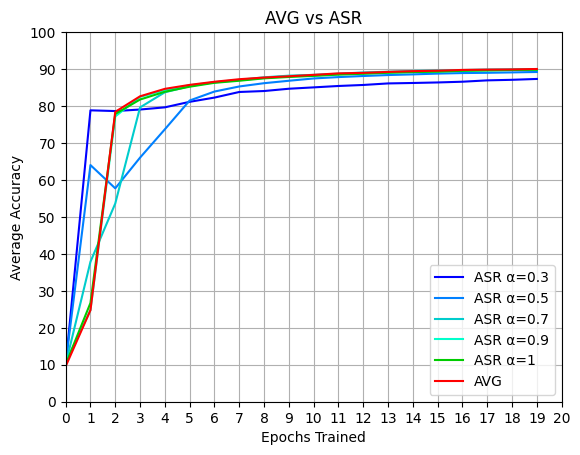
\includegraphics{ex1}

The lower values of ASR increase performance faster at the start, but then struggle to achieve the same perf as the higher values/AVG after some time. Hypothesis: this is because nodes become de-synced, then the amount of change per epoch is greater than the change per sync, so networks stay at local minima.

AVG performs the same as ASR 0.9 because there are 10 nodes, therfor they are mathematically identical.

ASR 1 performs very well too. Hypothesis: As model updates are sent before the sync step, no training is being lost, as all training done in this step is being stored on neighbour nodes.

From now on, ASR 0.9 will be used. It provides the same performance as AVG when in a dense network, but hypothetically will provide more stability when used in a sparse network with varying numbers of neighbours.

\subsection{Combination Methods: Varying $\beta$}
The purpose of this experiment is to find the relationship between $\beta$ and performance. Below are some details of the experiment:

\begin{itemize}
	\item All nodes were started at the same time
	\item ASR 0.9 was used
	\item The parameter $\beta$ varied
	\item The parameter $\gamma$ was set to 8
	\item The network is dense
\end{itemize}